\documentclass{beamer}

% For more themes, color themes and font themes, see:
% http://deic.uab.es/~iblanes/beamer_gallery/index_by_theme.html
%
\mode<presentation>
{
  \usetheme{Antibes}       % or try default, Darmstadt, Warsaw, ...
  \usecolortheme{dolphin} % or try albatross, beaver, crane, ...
  \usefonttheme{serif}    % or try default, structurebold, ...
  \setbeamertemplate{caption}[numbered]
  \setbeamertemplate{page number in head/foot}[framenumber]
  \setbeamertemplate{navigation symbols}{\footnotesize\usebeamertemplate{page number in head/foot}}
  \pgfdeclareimage[height=1cm]{logo}{images/constraint}
  \logo{\pgfuseimage{logo}}

}

\usepackage[ruled,vlined]{algorithm2e}
\usepackage[english]{babel}
\usepackage[utf8x]{inputenc}
\usepackage{ dsfont }
\usepackage{ bm }
\usepackage{mathtools}          %loads amsmath as well
\DeclarePairedDelimiter\Floor\lfloor\rfloor
\DeclarePairedDelimiter\Ceil\lceil\rceil

\usepackage{amsmath}
\DeclareMathOperator*{\argmax}{arg\,max}
\DeclareMathOperator*{\argmin}{arg\,min}
\newcommand{\norm}[1]{\left\lVert#1\right\rVert}
\AtBeginSection[]{
  \begin{frame}
  \vfill
  \centering
  \begin{beamercolorbox}[sep=8pt,center,shadow=true,rounded=true]{title}
    \usebeamerfont{title}\secname\par%
  \end{beamercolorbox}
  \vfill
  \end{frame}
}
\usepackage{hyperref}

% On Overleaf, these lines give you sharper preview images.
% You might want to `comment them out before you export, though.
\usepackage{pgfpages}
\pgfpagesuselayout{resize to}[%
  physical paper width=8in, physical paper height=6in]

% Here's where the presentation starts, with the info for the title slide
\author{Chapter 6: Constraint Satisfaction Problems}

\title{}

\subtitle{}
\date{}



\begin{document}

\begin{frame}
  \titlepage
\end{frame}

\begin{frame}{Components of a CSP}

    \begin{enumerate}
        \item A set of variables $\mathcal{X} = \left\{ X_1, X_2, \dots, X_n\right\}$
        \item A domain for each variable $\mathcal{D} = \left\{ D_1, D_2, \dots, D_n\right\}$
        \begin{itemize}
            \item $D_i$ is a set of allowable values $\{v_1, v_2, \dots, v_k\}$ for 
            variable $X_i$.
        \end{itemize}
        \item A collection of constraints $\mathcal{C}$
        \begin{itemize}
            \item A constraint $C_j$ is the pair 
            $\langle \texttt{scope}, \texttt{rel} \rangle$
            where the \texttt{scope} is the tuple of variables involved in the constraint, 
            and \texttt{rel} is the function that checks whether a tuple of values satisfies $C_j$.
        \end{itemize}
    \end{enumerate}

    \small
    Variable {\bf assignments} are consistent if the values assigned to the 
    variables don't violate any constraints. A {\bf complete assignment} provides
    a value for each variable. A {\bf CSP solution} is a consistent, complete assignment. A consistent, partial assignment is a partial solution. Partial solutions allow us to eliminate large groups of variable values from further 
    consideration, and in this way CSP formulations can help produce computationally
    efficient searches.
    
\end{frame}

\begin{frame}{A simple constraint}
    Suppose you have variables $(X_1, X_2)$ that for which
    $D_1 = D_2 = \{1, 2, 3\}$.

    \vspace{.1in}

    The constraint $X_1>X_2$ is written formally as either

    \[\langle (X_1, X_2), X_1 > X_2 \rangle\]

    or 

    
    \[\langle (X_1, X_2), \{(3,1), (3,2), (2,1)\} \rangle\]

    
\end{frame}

\begin{frame}{A map coloring example}

    \begin{figure}
        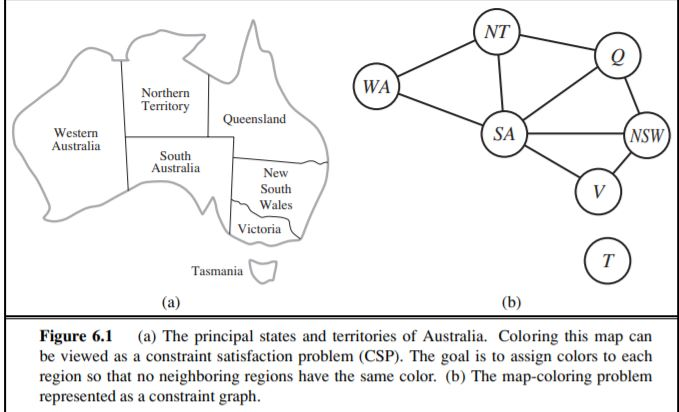
\includegraphics[width=10cm]{images/map_coloring}
    \end{figure}
    
\end{frame}

\begin{frame}{A map coloring example as a CSP}

    \begin{figure}
        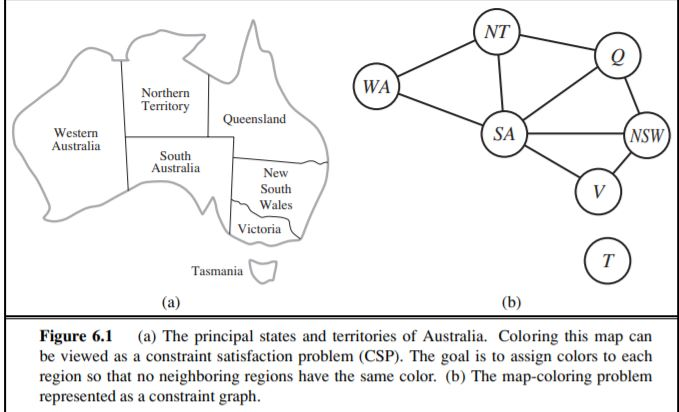
\includegraphics[width=5cm]{images/map_coloring}
    \end{figure}
The variables are
    $$\mathcal{X} = \{WA, NT, Q, NSW, V, SA, T\}$$
and each one can assume the colors
$$ D = \{\texttt{red}, \texttt{green}, \texttt{blue}\}$$
with the constraint that neighbors must have unique colors:
$$\mathcal{C}= \left \{ \langle \{SA, WA\}, SA \neq WA \rangle, 
\langle \{ SA, NT\}, SA \neq NT\rangle, \dots \right\}$$


    
\end{frame}

\begin{frame}{A map coloring exercise from Chegg}

    \begin{figure}
        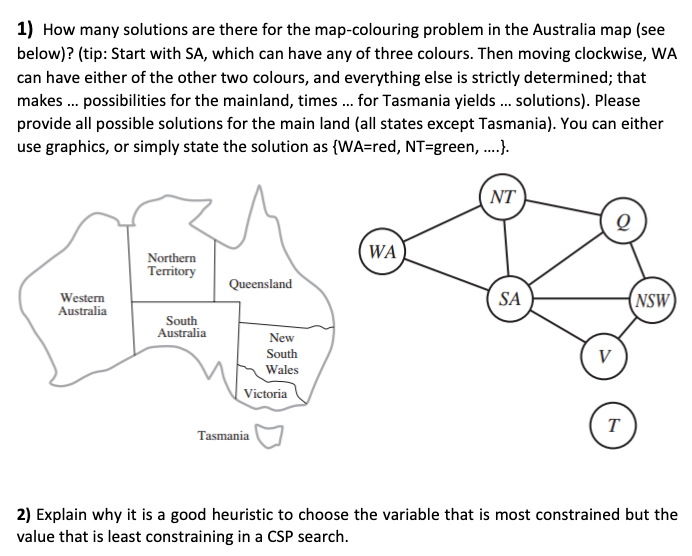
\includegraphics[width=9cm]{images/map_coloring_2}
    \end{figure}
    
\end{frame}

\begin{frame}{CSP flavors}
    Types of domains
    \begin{itemize}
        \item Discrete, finite domains
        \item Discrete, infinite domains (e.g. constraints on integer variables is {\bf integer programming})
        \item Linear constraints on continuous domains ({\bf linear programming})
    \end{itemize}

    Types of constraints
    \begin{itemize}
        \item {\bf unary} constraints act on one variable
        \item {\bf binary} constraints act on two variables
        \item {\bf ternary} constraints $\dots$
        \item {\bf global} constraints act on an arbitrary subset of variables 
    \end{itemize}
    
\end{frame}

\begin{frame}{Examples of global constraints}
\texttt{Alldiff} is the constraint that all variable values must differ

\vspace{.1in}

{\bf Cryptarithmetic} puzzles use an \texttt{Alldiff} constraint
    \begin{figure}
        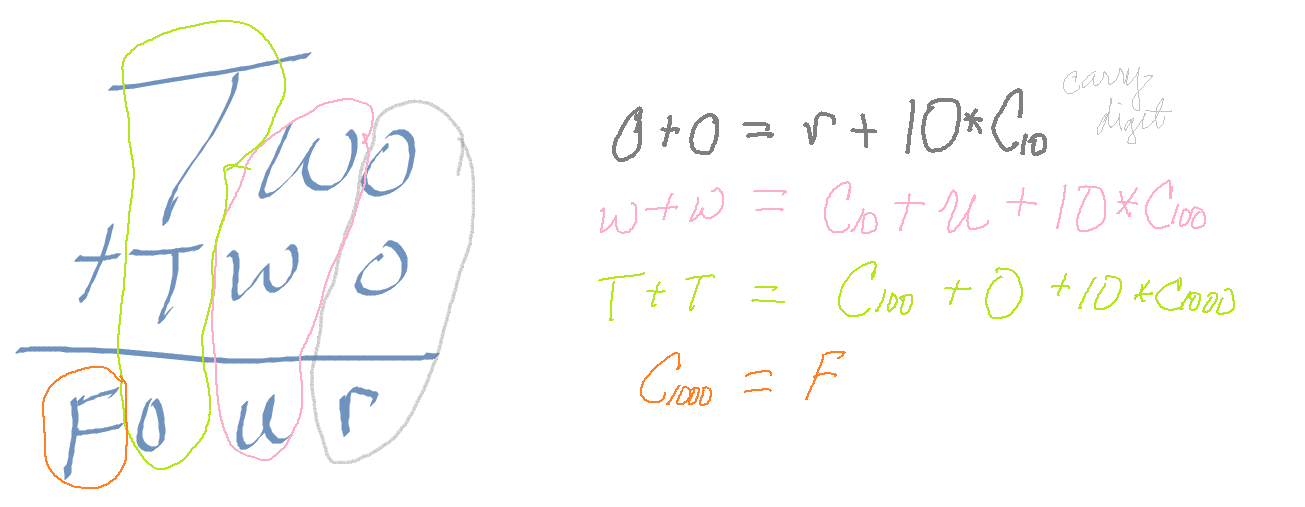
\includegraphics[width=9cm]{images/two_two_four.png}
    \end{figure}
\end{frame}

\begin{frame}{The constraint hypergraph}
   \begin{figure}
       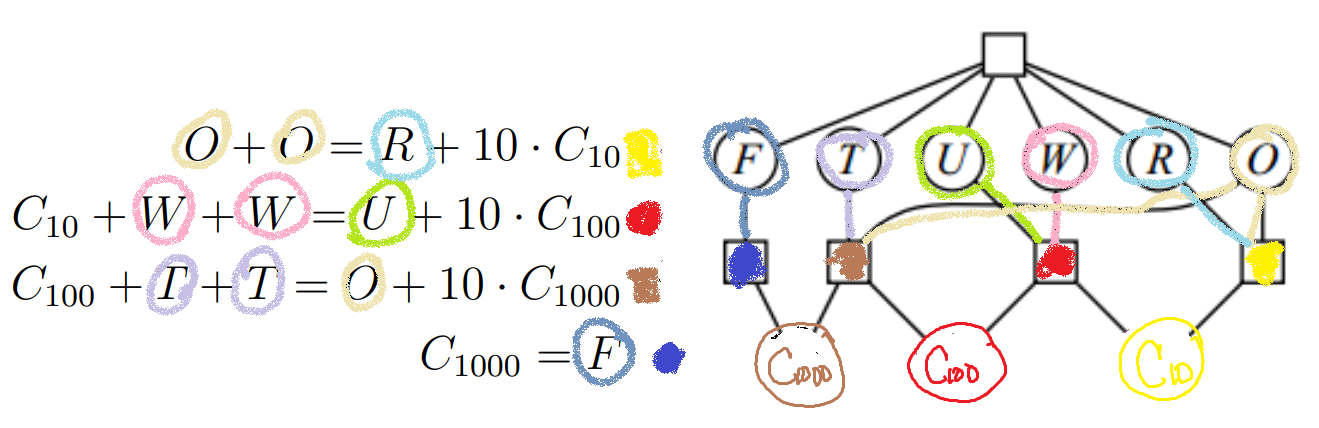
\includegraphics[width=10cm]{images/constraint_hypergraph}
   \end{figure} 

   The top square is the initial \texttt{Alldiff} constraint,
   and each additional square represents another constraint. The carry 
   digits become extra variables that had to be introduced (and do not have to be 
   distinct).
\end{frame}

\begin{frame}{Every finite-domain constaint can be reduced to a set of binary constraints}
\small
    One non-intuitive way to do this is to create a new {\bf dual} problem that
    has the constraints as variables

    \begin{align*}
       \mathcal{X} &= \{X, Y, Z\} \\
       D_X = D_Y = D_Z &= \{1, 2, 3, 4, 5\} \\
       C_1 &= \langle(X,Y, Z), X + Y = Z  \rangle \\
       C_2 &= \langle (X,Y), X + 1 = Y \rangle
    \end{align*}
    
    \begin{align*}
       \mathcal{X} &= \{C_1, C_2\} \\
       D_{C_1} &= \{ (X, Y, Z) \in \{1, 2, 3, 4, 5\} \, | \, X + Y = Z \} \\
       D_{C_2} &= \{ (X, Y) \in \{1, 2, 3, 4, 5\} \,|\, X + 1 = Y \}\\
       C &= \langle(C_1, C_2), R \rangle
    \end{align*}

    The relation $R$ contains the variables that co-satisfy $C_1$ and $C_2$ 

    $$
    R = \{ ((1, 2, 3, 1, 2)), ((2, 3, 5), (2, 3))\}
    $$

    
\end{frame}

\begin{frame}[t]{Every finite-domain constaint can be reduced to a set of binary constraints}
\small
How would you choose to turn this into only binary constraints?

    \begin{align*}
       \mathcal{X} &= \{X, Y, Z\} \\
       D_X = D_Y = D_Z &= \{1, 2, 3, 4, 5\} \\
       C_1 &= \langle(X,Y, Z), X + Y = Z  \rangle \\
       C_2 &= \langle (X,Y), X + 1 = Y \rangle
    \end{align*}
    
\end{frame}

\begin{frame}{Constraint Propagation}
    Again, the power of a CSP is that every time you enforce one constraint,
    you reduce the number of legal values for at least some of the variables.
    Propagation through constraints could solve the whole problem, or perhaps
    reduce the variables that are still needed to be considered if there are multiple domain values remaining for each variable. (Note: a solution may not be unique.)

    \vspace{.1in}

    One strategy is {\bf local consistency} in which {\em each variable is a node
    in a graph} and {\em each binary constraint is an edge in the graph}.

    \vspace{.1in}

    On the previous slide, draw the associated graph.    
\end{frame}

\begin{frame}{Node consistency}
    Each node's domain must satisfy any unary constraints.

    \small
    \begin{figure}
        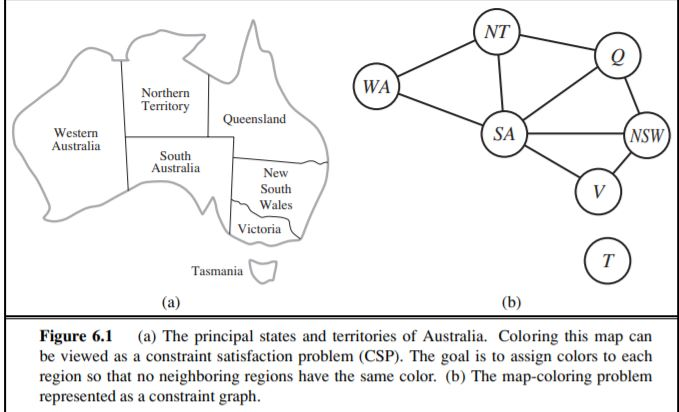
\includegraphics[width=5cm]{images/map_coloring}
    \end{figure}
The variables are
    $$\mathcal{X} = \{WA, NT, Q, NSW, V, SA, T\}$$
$$ D = \{\texttt{red}, \texttt{green}, \texttt{blue}\}$$

As a silly example, suppose we know SA hates \texttt{green}. Then we 
could start with 

$$D_{SA} = \{\texttt{red}, \texttt{blue} \}$$

\end{frame}

\begin{frame}{Arc Consistency}

    The variable $X_i$ is {\bf arc-consistent} with variable $X_j$ if 
    for each binary constraint $C$ with scope $(X_i, X_j)$ and 
    each value $v_i \in D_i$ there exists $v_j \in D_j$ such that
    $C$ is satisfied.

    \vspace{.1in}

    By applying the rule of arc consistency, we can reduce the domain for a 
    problem. For example, return to the map coloring problem in the 
    previous slide. When we applied the unary constraint to SA, does 
    arc consistency allow any other domain reductions? 
    
\end{frame}

\begin{frame}{Arc consistency Example}
    Let's think through what can be deduced using arc consistency.

    \begin{figure}
        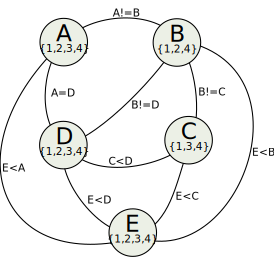
\includegraphics[width=6cm]{images/boris_arc_consistency}
    \end{figure}

    \tiny{from boristhebrave.com}
    
\end{frame}

\begin{frame}{AC3: Popular Arc Consistency Algorithm}

    \texttt{Queue}: Two arcs (bidirectional) for each binary constraint

    \vspace{.1in}
    Choose an arc to consider.
    \begin{itemize}
        \item If the arc doesn't change any domains, move on to the next arc.
        \item If the arc {\em does} change a domain $D_i$, then add all arcs to 
        adjacent nodes back in (if they aren't already there). 
        
        
        AC3's worst-case complexity is $\mathcal{O}(cd^3)$ where $c$ is the number of 
        constraints and $d$ is the maximum domain size.
    \end{itemize}
\end{frame}

\begin{frame}{Path consistency}
    \small
    Rather than just considering binary constraints, pairs of binary constraints
    are considered by looking at triples of variables. The pair $\{X_i, X_j\}$ is 
    {\bf path consistent} with $X_m$ if for any pair $(a, b)$ that satisfies 
    the binary constraint(s) for $\{X_i, X_j\}$ there exists a value $c \in D_m$ that satisfies any binary constraint(s) between $X_i$ and $X_m$ as well as between $X_j$ and $X_m$.
    
    
    How would this help us with the coloring problem if we assume there are only two colors?

    \begin{figure}
        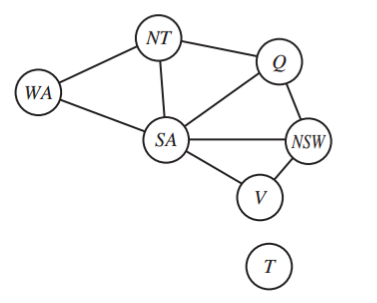
\includegraphics[width=7cm]{images/map_graph}
    \end{figure}
    
\end{frame}

\begin{frame}{$k$-consistency}

    This is an extension of the idea of path consistency. 
    A CSP is $k$-consistent if for any consistent assignment for $k-1$ variables, a consistent assignment can always be made for a $k$th variable.

    \vspace{.1in}

    A CSP is {\bf strongly $k$-consistent} if it $k, (k-1)-, (k-2)-, \cdots 1-$consistent.

    \vspace{.1in}

    In practice, going for more than path consistency is a very expensive approach.

\end{frame}

\begin{frame}[t]{Another global constraint: Resource constraints}

    An example of a resource constraint is \texttt{Atmost}. 

    \vspace{.1in}
    Application: Suppose $P_1$, $P_2$, $P_3$, and $P_4$ people are assigned to four tasks, but that we're not allowed to hire more than 10 people in total. This global resource constraint would be written as 
    $$\texttt{Atmost}(10, P_1, P_2, P_3, P_4)$$

    \vspace{.1in}
    Given the \texttt{Atmost} constraint, how would you edit the shared
    domain $\{2, 3, 4, 5, 6\}$?

    
\end{frame}

\begin{frame}{Large problem domains and bounds propagation}
    If we extended the above problem to a large company, we can't 
    list every integer value for the number of personnel, and we 
    would instead enumerate domains using interval notation. As we 
    apply consistency rules and adjust the domains, we apply {\bf bounds
    propagation} and perhaps raise the 
    lower bounds and decrease the upper bounds for domains to make them {\bf bounds consistent}.

\end{frame}

\begin{frame}[t]{Let's list some constraints for a Sudoku puzzle}
    \begin{figure}
        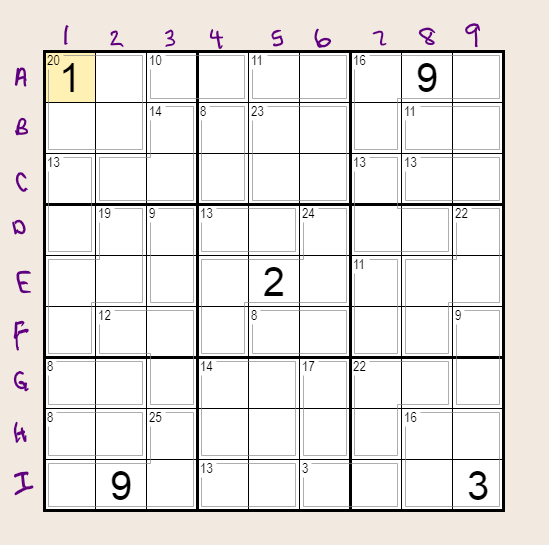
\includegraphics[width=5cm]{images/sudoku}
    \end{figure}

    
\end{frame}

\begin{frame}{How big is a search?}
    \small

    \begin{figure}
        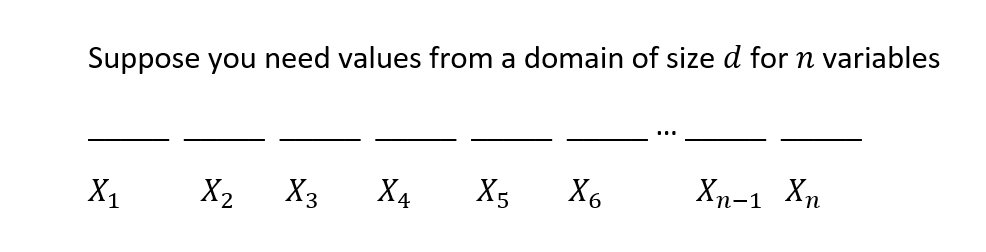
\includegraphics[width=10cm]{images/csp_search}
    \end{figure}

    If you were to create a search tree, you'd want to first choose one
    value. So you'd choose one variable ($n$ choices) to assign, and you'd
    give it one of the $d$ domain values. There are therefore $kn$ ways to start 
    this tree.

    \vspace{0.1in}

    At the next tree level, there are only $n-1$ choices remaining, so there are
    $k(n-1)$ choices for the next level. Continuing this logic, we see that
    the size of our search tree is $n!d^n$.

    \vspace{0.1in}

    However, look at the blanks. How many possible assignments are there? Clearly
    this is a terrible search tree idea.
    
\end{frame}

\begin{frame}{Why do we teach CS majors combinatorics?}
\small
    How many 4-letter ``words" can we create from the letters in FLOWERS?

    \vspace{1in}
    How many collections of 4 letters can we choose from the letters in FLOWERS?
    
    \vspace{1in}
    The moral is, no one cares which variable I pick first, second, and so on. So no one cares which of the $n$ variables I start with. Just pick one and give it a value and move down a layer in the tree. There are only $d^n$ leaves in this search tree. 

\end{frame}

\begin{frame}{Backtracking-search}
    \begin{enumerate}
        \item Choose an unassigned variable.
        \item For each consistent value in its domain, try to extend this to a solution by calling backtracking-search on the solution that uses this value.
        \begin{itemize}
            \item If the call succeeds, the solution is returned.
            \item If the call fails, we try the next value.
        \end{itemize}
        \item If we run out of values with no solution we return failure.
    \end{enumerate}
    
    
\end{frame}

\begin{frame}{Variable order matters in a search}
    Unassigned variable ordering approaches
    \begin{itemize}
        \item {\bf Minimum-remaining-values (MRV)}: This is the most effective
        way to prune the search tree early on by using this bottleneck to identify failures down the line.
        \item {\bf Degree heuristic}: If all of the consistent domains are the same size, MRV doesn't help. Start with the variable that is involved in 
        the largest number of constraints involving other variables.
    \end{itemize}

    In what order should we explore values?

    \begin{itemize}
        \item {\bf Least-constraining value heuristic}: Test all values against the the neighbors -- variables that share constraints -- and work further down the tree by using the value that eliminated the fewest number of values from its neighbors.
    \end{itemize}
    
\end{frame}

\begin{frame}{Which choice is the least constraining value?}

    \begin{figure}
        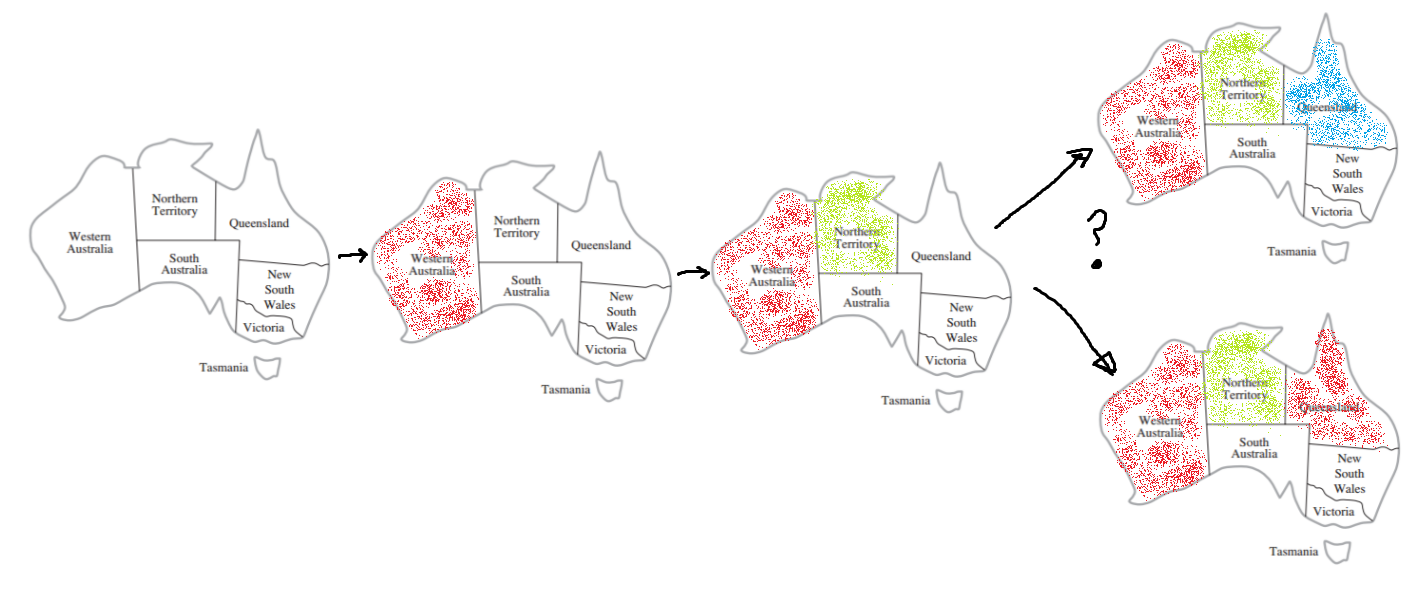
\includegraphics[width=10cm]{images/least_constraing_value.png}
    \end{figure}
    
\end{frame}

\begin{frame}{Making CSP search faster}
    \begin{itemize}
        \item {\bf Forward checking}: Once you choose a variable value, perform consistency checking for each variable connected to the originating variable by a constraint.  Note that without this inference, we'd only check the {\em next} variable we chose, and many possible eliminations would be missed.
        \item {\bf Maintaining Arc Consistency (MAC)}: In the previous graph, only the red choice for Queensland allows arc consistency moving forward. MAC alters the AC3 algorithm by searching constraint-neighbor arcs first after a value has been assigned. For example, on the previous slide if I put blue in Queensland, I wouldn't jump to color Victoria next. Rather, I'd want to check whether that 
        would work for my constraint neighbors.
    \end{itemize}
\end{frame}

\begin{frame}{Is there a smarter way to back up?}
    When we fail in AC3, we just back up and try the next variable. But what if the reason
    this failed was that the variable {\em before} this one was a terrible choice? Then I'll do a zillion failures, exhausting all possible choices for the current variable before I back up further.

    \vspace{0.1in}
    Other approches:
    \begin{itemize}
        \item {\bf Backjumping} figures out a smarter ``jump'' to a higher part of the tree that is most likely to be the culprit of the lack of consistency. There are three flavors of this:
        \begin{itemize}
            \item Gaschnig's Backjumping: focus on the earliest chosen value that conflicts with the current proposed value and jump to that choice in the tree
            \item Graph-based Backjumping: focus on the parent variables (not values) in 
            the constraint graph to decide where to jump
            \item Conflict-directed Backjumping: combine information from the constraint 
            graph with the minimal prefix conflict set from Gaschnig.
        \end{itemize}

        \item {\bf No-good learning} tries to understand why there was a dead-end, and 
        seeks to predict those sooner.
    \end{itemize}
    
\end{frame}

\begin{frame}{Structuring your problem for a quick solution}

    In the coloring problem, each {\bf connected component} has a coloring scheme
    that is independent of other components. So one way to reduce a problem is to split it into its connected components.

    \vspace{.1in}

    But how often is that going to happen?
    
\end{frame}

\begin{frame}{Tree constraint graphs}
    \begin{figure}
        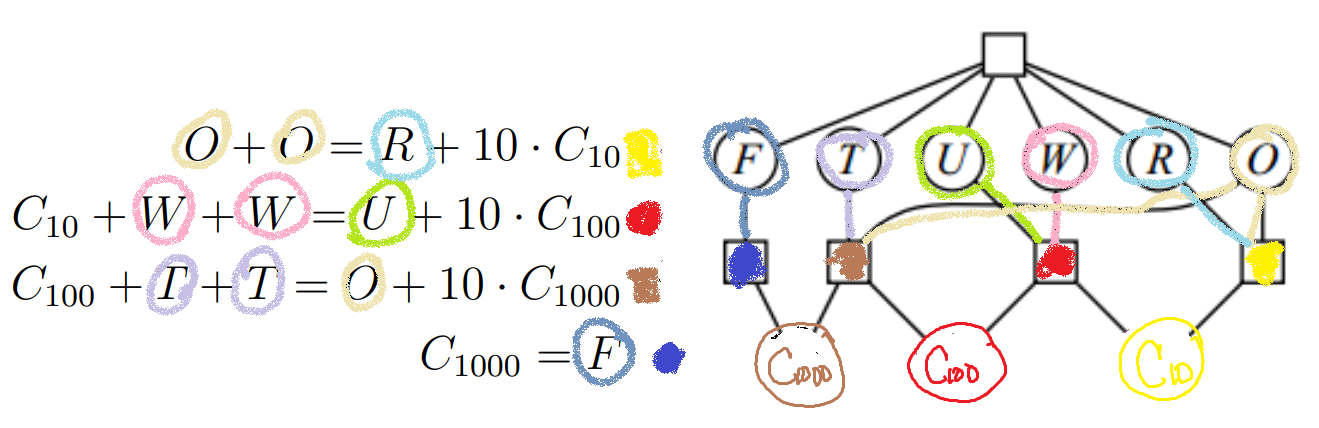
\includegraphics[width=8cm]{images/constraint_hypergraph}
    \end{figure} 

    Remember our constraint graph for the Cryptarithmetic example? Look how ``O'' has two constraints, and thus paths to T and R, as well as our invented variables.

    \vspace{.1in}

    A constraint graph is a {\bf tree} when any two variables are connected by only one path. Such CSPs can be solved in $\mathcal{O}(\text{\# vars})$.
\end{frame}

\begin{frame}{Why are tree graphs better?}
    A CSP has {\bf directional arc consistency (DAC)} under an ordering of the variables 
    $X_1, X_2, \dots X_n$ if and only if every $X_i$ is arc-consistent with each $X_j$ that follows it.

    \vspace{0.1in}
    The tree is created by performing a topological sort on its constraint graph -- this sort should preserve order, allowing skips.

    \begin{figure}
        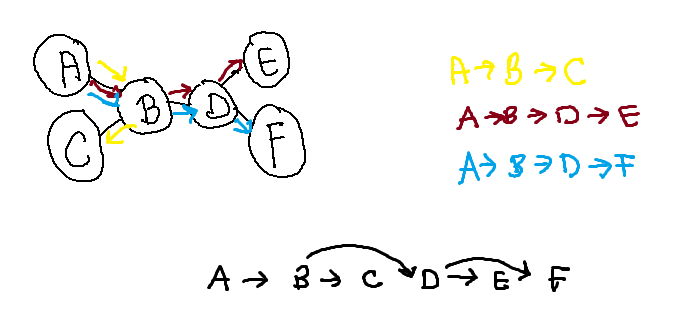
\includegraphics[width=8cm]{images/top_sort_2}
    \end{figure}
    
\end{frame}

\begin{frame}{Another topological sort}

    \begin{figure}
        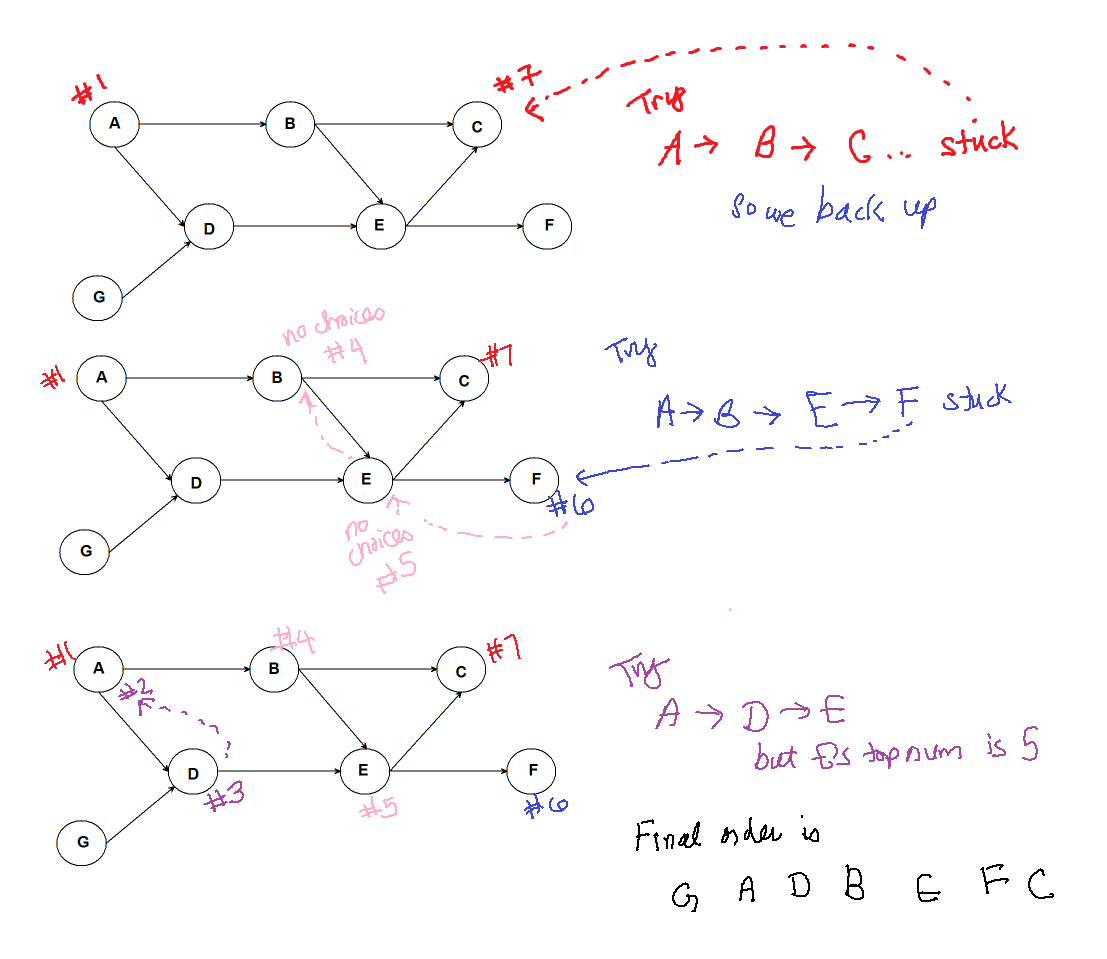
\includegraphics[width=9cm]{images/top_sort_1}
    \end{figure}
    
\end{frame}

\begin{frame}{How does the topological sort help?}
    Now the tree can obtain DAC in $\mathcal{O}(n)$ steps. Each step compares up to $d$ possible values for a pair of variables, so the overall computation is 
    $\mathcal{O}(nd^2)$.

    \vspace{0.1in}
    Because the graph is arc consistent, we now just choose the solution by choosing any remaining value as we walk down the tree. We never have to backtrack.
    
\end{frame}

\begin{frame}{Is our Australia problem a tree?}
    \begin{figure}
        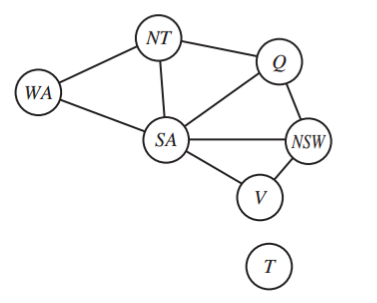
\includegraphics[width=7cm]{images/map_graph}
    \end{figure}
    
\end{frame}

\begin{frame}{What would it take to make our Australia problem a tree?}
    \begin{figure}
        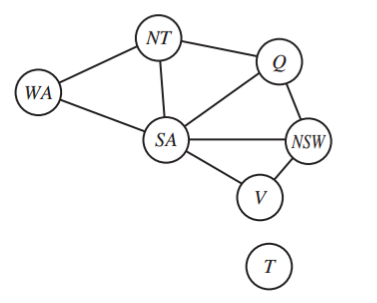
\includegraphics[width=7cm]{images/map_graph}
    \end{figure}
    
\end{frame}

\begin{frame}{Cutset conditioning}
    \begin{itemize}
        \item Choose a subset $S$ of CSP's variables so that the graph with those
        variables removed is a tree. $S$ is called a {\bf cycle subset.}
        \item Create a list of assignments within $S$ that achieve consistency within $S$. For set assignment set
        \begin{itemize}
            \item Remove inconsistent values from the variables in $CSP\setminus S$.
            \item If the remaining graph has a solution, return that solution along with the assignments for $S$.
        \end{itemize}
    \end{itemize}
    
\end{frame}

\end{document}